\documentclass[11pt]{scrartcl}

\usepackage[top=2cm]{geometry}
\usepackage{url}
\usepackage{tikz}

\title{
  \textbf{\large Database Management and Tuning -- Assignment 7}\\
  Transaction Chopping
}

\author{
 Group Name A3\\
 \large Platzer Hugo, 1421579 \\
 \large Strohmeier Mario, 1422959
}

\begin{document}

\maketitle

{\it Notes:}

\begin{itemize}
\item The chopping graphs may also be drawn by hand and attached as a
  hard copy on paper. In the case of drawings on paper, you need to
  hand in the drawings during the lab.
\item The chopping graphs need to show all S- and C-edges, and you
  need to cross out (or otherwise mark) the S-edges that must be
  removed to get a correct chopping. Also show the write list for each
  chopping graph.
\end{itemize}

\section*{Task 1:  Bank Accounts}

\subsection*{(a) SQL Queries}

{\it Give the SQL queries (including pseudo code if necessary) for each
transaction.}

\paragraph{Transaction T1}

{\small
\begin{verbatim}
...
\end{verbatim}
}

\paragraph{Transaction T2}

{\small
\begin{verbatim}
...
\end{verbatim}
}

\paragraph{Transaction T3}

{\small
\begin{verbatim}
...
\end{verbatim}
}

\subsection*{(b) Model Transactions}

{\it Model all transactions with read/write operations.}

\smallskip

{\it Note: Define the data items first, for example, $a_1$ is
   account\,1, $b_1$ is branch\,1, etc. Define the minimum number of
  data items that represent all possible conflicts in the scenario.}

\begin{enumerate}
\item[T1:]
\item[T2:]
\item[T3:] 
\end{enumerate}

\subsection*{(c) Chopping Graph}

{\it Show the chopping graph and give the finest possible correct
  chopping.}

\medskip

\noindent
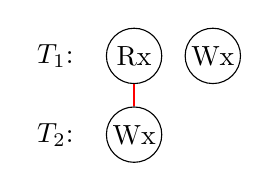
\begin{tikzpicture}[every node/.style={draw,circle,minimum size=2em,inner sep=1}]
\node[draw=none] (T1) at (0, 0) {$T_1$:};
\node (T1_1) at (1, 0) {Rx};
\node (T1_2) at (2, 0) {Wx};
\node[draw=none] (T2) at (0, -1) {$T_2$:};
\node (T2_1) at (1, -1) {Wx};

\draw[draw=red,line width=1pt] (T1_1) -- (T2_1);
\end{tikzpicture}

\medskip

\noindent Finest correct chopping:
\begin{enumerate}
\item[T1:]
\item[T2:]
\item[T3:] 
\end{enumerate}

\subsection*{(d) Two Transactions Update the Same Account}

{\it How does the chopping change if two concurrent transactions of type
$T_1$ can update the same account? Explain.}

\subsection*{(e) Order of Atomic Operations}

{\it The order of the atomic operations in $T_3$ has an impact on the
  chopping. Show two semantically equivalent implementations of $T_3$,
  one which favors chopping, the other which does not favor
  chopping. Explain.}


\section*{Task 2: Chopping Graphs}

\subsection*{(a) All Transactions}

\medskip

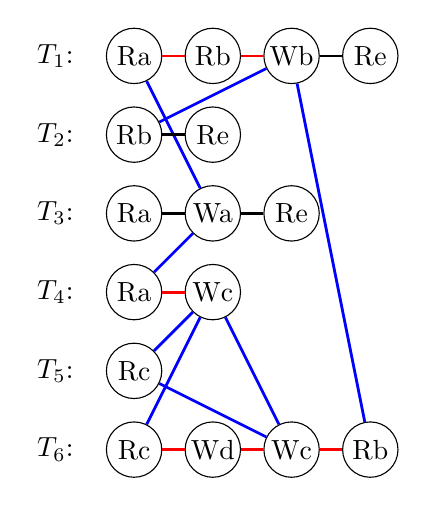
\begin{tikzpicture}[every node/.style={draw,circle,minimum size=2em,inner sep=1}]
\node[draw=none] (T1) at (0, 0) {$T_1$:};
\node (T1_1) at (1, 0) {Ra};
\node (T1_2) at (2, 0) {Rb};
\node (T1_3) at (3, 0) {Wb};
\node (T1_4) at (4, 0) {Re};
\node[draw=none] (T2) at (0, -1) {$T_2$:};
\node (T2_1) at (1, -1) {Rb};
\node (T2_2) at (2, -1) {Re};
\node[draw=none] (T3) at (0, -2) {$T_3$:};
\node (T3_1) at (1, -2) {Ra};
\node (T3_2) at (2, -2) {Wa};
\node (T3_3) at (3, -2) {Re};
\node[draw=none] (T4) at (0, -3) {$T_4$:};
\node (T4_1) at (1, -3) {Ra};
\node (T4_2) at (2, -3) {Wc};
\node[draw=none] (T5) at (0, -4) {$T_5$:};
\node (T5_1) at (1, -4) {Rc};
\node[draw=none] (T6) at (0, -5) {$T_6$:};
\node (T6_1) at (1, -5) {Rc};
\node (T6_2) at (2, -5) {Wd};
\node (T6_3) at (3, -5) {Wc};
\node (T6_4) at (4, -5) {Rb};

\draw[draw=red,line width=1pt] (T1_1) -- (T1_2);
\draw[draw=red,line width=1pt] (T1_2) -- (T1_3);
\draw[line width=1pt] (T1_3) -- (T1_4);
\draw[draw=blue,line width=1pt] (T1_1) -- (T3_2);
\draw[draw=blue,line width=1pt] (T1_3) -- (T2_1);
\draw[draw=blue,line width=1pt] (T1_3) -- (T6_4);
\draw[line width=1pt] (T2_1) -- (T2_2);
\draw[line width=1pt] (T3_1) -- (T3_2);
\draw[line width=1pt] (T3_2) -- (T3_3);
\draw[draw=blue,line width=1pt] (T3_2) -- (T4_1);
\draw[draw=red,line width=1pt] (T4_1) -- (T4_2);
\draw[draw=blue,line width=1pt] (T4_2) -- (T5_1);
\draw[draw=blue,line width=1pt] (T4_2) -- (T6_1);
\draw[draw=blue,line width=1pt] (T4_2) -- (T6_3);
\draw[draw=blue,line width=1pt] (T5_1) -- (T6_3);
\draw[draw=red,line width=1pt] (T6_1) -- (T6_2);
\draw[draw=red,line width=1pt] (T6_2) -- (T6_3);
\draw[draw=red,line width=1pt] (T6_3) -- (T6_4);
\end{tikzpicture}

\medskip

\noindent Finest correct chopping:
\begin{enumerate}
\item[T11:]Ra,Rb,Wb, T12: Re
\item[T21:]Rb, T22: Re
\item[T31:]Ra, T32: Wa, T33: Re
\item[T4:]Ra,Wc
\item[T5:]Rc
\item[T6:]Rc,Wd,Wc,Rb
\end{enumerate}


\subsection*{(b) All Transactions Except T4}

\medskip

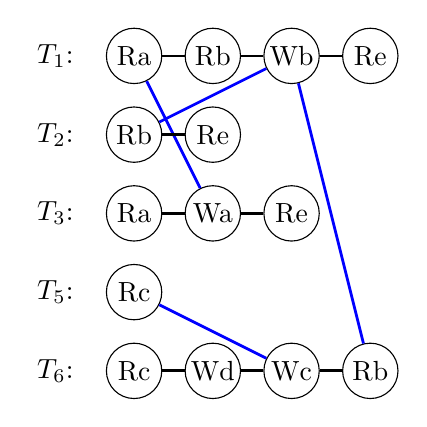
\begin{tikzpicture}[every node/.style={draw,circle,minimum size=2em,inner sep=1}]
\node[draw=none] (T1) at (0, 0) {$T_1$:};
\node (T1_1) at (1, 0) {Ra};
\node (T1_2) at (2, 0) {Rb};
\node (T1_3) at (3, 0) {Wb};
\node (T1_4) at (4, 0) {Re};
\node[draw=none] (T2) at (0, -1) {$T_2$:};
\node (T2_1) at (1, -1) {Rb};
\node (T2_2) at (2, -1) {Re};
\node[draw=none] (T3) at (0, -2) {$T_3$:};
\node (T3_1) at (1, -2) {Ra};
\node (T3_2) at (2, -2) {Wa};
\node (T3_3) at (3, -2) {Re};
\node[draw=none] (T5) at (0, -3) {$T_5$:};
\node (T5_1) at (1, -3) {Rc};
\node[draw=none] (T6) at (0, -4) {$T_6$:};
\node (T6_1) at (1, -4) {Rc};
\node (T6_2) at (2, -4) {Wd};
\node (T6_3) at (3, -4) {Wc};
\node (T6_4) at (4, -4) {Rb};

\draw[line width=1pt] (T1_1) -- (T1_2);
\draw[line width=1pt] (T1_2) -- (T1_3);
\draw[line width=1pt] (T1_3) -- (T1_4);
\draw[draw=blue,line width=1pt] (T1_1) -- (T3_2);
\draw[draw=blue,line width=1pt] (T1_3) -- (T2_1);
\draw[draw=blue,line width=1pt] (T1_3) -- (T6_4);
\draw[line width=1pt] (T2_1) -- (T2_2);
\draw[line width=1pt] (T3_1) -- (T3_2);
\draw[line width=1pt] (T3_2) -- (T3_3);
\draw[draw=blue,line width=1pt] (T5_1) -- (T6_3);
\draw[line width=1pt] (T6_1) -- (T6_2);
\draw[line width=1pt] (T6_2) -- (T6_3);
\draw[line width=1pt] (T6_3) -- (T6_4);
\end{tikzpicture}

\medskip

\noindent Finest correct chopping:
\begin{enumerate}
\item[T11:]Ra, T12: Rb, T13: Wb, T14: Re
\item[T21:]Rb, T22: Re
\item[T31:]Ra, T32: Wa, T33: Re
\item[T5:]Rc
\item[T61:]Rc, T62: Wd, T63: Wc, T64: Re
\end{enumerate}


\subsection*{Time Spent on this Assignment}

Time in hours: {\bf XXX}

% \bigskip

% \begin{center}
%   \begin{tabular}{c}
%     \hline
%     {\bf Important:} Reference your information sources!
%     \\\hline
%   \end{tabular}
% \end{center}

\end{document}
